% Guia de Estudo (PT-PT) — CLARION: da estaca zero à defesa
% Beamer -> PDF. Deck VISUAL e progressivo que ENSINA (não resume).
% Honestidade: só conceitos/código/números reais da tese; a tese NÃO treina modelos nem usa visão
% computacional (usa SBERT pré-treinado + estatística + recuperação + XAI).
% Construído por partes: P0 (capa/como usar) + P1 (IA do zero, só o que a tese usa) + glossário.
\documentclass[aspectratio=169,11pt]{beamer}
\usetheme{Madrid}
\usecolortheme{seahorse}
\usepackage[utf8]{inputenc}
\usepackage[T1]{fontenc}
\usepackage{booktabs}
\usepackage{amsmath}
\usepackage{tikz}
\usetikzlibrary{positioning, arrows.meta, calc, fit, backgrounds, shapes.geometric}
% Nos diagramas, nunca cortar palavras a meio (quebrar só em espaços).
\tikzset{every node/.append style={execute at begin node={\hyphenpenalty=10000\exhyphenpenalty=10000\relax}}}
% Sem babel-PT neste ambiente: linhas curtas de slide, desligar hifenização para não cortar mal as palavras.
\hyphenpenalty=10000 \exhyphenpenalty=10000
\graphicspath{{../../thesis/figures/}}
\setbeamertemplate{navigation symbols}{}
\setbeamertemplate{caption}{\raggedright\insertcaption\par}
\setbeamertemplate{itemize items}[circle]

% atalhos de cor para destacar
\definecolor{good}{RGB}{30,120,60}
\definecolor{bad}{RGB}{170,40,40}
\newcommand{\key}[1]{\textbf{\structure{#1}}}

\title[Guia de Estudo: CLARION]{Guia de Estudo --- CLARION}
\subtitle{Da estaca zero à defesa: aprender a tese como se a tivesse escrito}
\author[H.\ Santos]{Henrique J.\ S.\ Santos \\ \footnotesize Orientador: Prof.\ Luís Gomes \quad Coorientador: Rafael Silva}
\institute[ISEP]{MEIA, Instituto Superior de Engenharia do Porto}
\date{\footnotesize Material de preparação para a defesa}

\begin{document}

\begin{frame}\titlepage\end{frame}

% ====================================================================
\section{Como usar}

\begin{frame}{Como usar este guia}
\begin{columns}[T]
\column{0.58\textwidth}
\begin{itemize}
  \item Foi feito para quem \key{não sabe nada de IA}. Começa do zero.
  \item \key{Uma ideia por slide.} Primeiro a \emph{intuição} (com analogias), só depois o detalhe.
  \item Lê \key{pela ordem}: cada parte prepara a seguinte.
  \item No fim, deves conseguir responder com confiança a "porquê isto?" em cada passo da tese.
\end{itemize}
\vspace{2mm}
\footnotesize Estuda este guia a par com a própria tese e com os slides de defesa (\texttt{slides/}).
\column{0.42\textwidth}
\begin{block}{O percurso}
\footnotesize
\begin{enumerate}
  \item IA do zero (só o que a tese usa)
  \item O problema e a contribuição
  \item O sistema (dados, partes, fluxo)
  \item Os dados, a olho
  \item O código, módulo a módulo
  \item Workflow ponta a ponta
  \item Avaliação e decisões
  \item Perguntas do júri
\end{enumerate}
\end{block}
\end{columns}
\end{frame}

\begin{frame}{A tese em três frases (o teu \emph{pitch})}
\begin{block}{Se só decorares isto, já defendes a ideia central}
\begin{enumerate}
  \item Construí o \key{CLARION}, um sistema que avisa um investidor de retalho quando há um \emph{movimento
        de mercado invulgar} ou uma \emph{notícia relevante}, e \key{explica} cada alerta de forma
        rastreável (evento, raciocínio, fontes, precedentes históricos).
  \item A contribuição é de \key{Engenharia de IA}: não inventei algoritmos; \emph{integrei, apliquei e
        avaliei criticamente} componentes existentes num sistema funcional, explicável e reproduzível.
  \item \key{Não prevejo preços.} Mostro o que aconteceu \emph{depois} de notícias parecidas no passado,
        como evidência, com honestidade sobre as limitações.
\end{enumerate}
\end{block}
\end{frame}

% ====================================================================
\section{IA do zero}

\begin{frame}{O que é Inteligência Artificial? E \emph{Machine Learning}?}
\begin{columns}[T]
\column{0.5\textwidth}
\key{Inteligência Artificial (IA)}\\
Fazer com que um computador resolva tarefas que pareceriam precisar de "inteligência" humana (decidir,
reconhecer, recomendar).
\vspace{3mm}

\key{Machine Learning (ML)}\\
Em vez de escrever \emph{regras} à mão, o computador \emph{aprende padrões a partir de dados}.
\column{0.5\textwidth}
\begin{block}{Analogia}
\footnotesize
\emph{Regras à mão:} explicar a alguém, passo a passo, como reconhecer um gato.\\[2mm]
\emph{ML:} mostrar mil fotos de gatos e deixar a pessoa aprender o padrão sozinha.
\end{block}
\vspace{1mm}
{\footnotesize Nesta tese, a "aprendizagem" já vem \key{pronta} (modelos pré-treinados). Ver o slide
seguinte.}
\end{columns}
\end{frame}

\begin{frame}{O que esta tese É --- e o que \key{NÃO} é (muito importante)}
\begin{columns}[T]
\column{0.5\textwidth}
\begin{block}{\textcolor{good}{O que usa}}
\footnotesize
\begin{itemize}
  \item Um \key{embedder de texto pré-treinado} (SBERT) --- só para \emph{usar}, não para treinar.
  \item \key{Estatística} simples (z-score: média e desvio-padrão).
  \item \key{Similaridade do cosseno} (comparar vetores).
  \item \key{Event study} (aritmética de retornos).
  \item Métricas de \key{recuperação} (precision@k).
  \item \key{Explicabilidade} (mostrar a evidência).
\end{itemize}
\end{block}
\column{0.5\textwidth}
\begin{block}{\textcolor{bad}{O que NÃO usa (e porquê)}}
\footnotesize
\begin{itemize}
  \item \textcolor{bad}{$\times$}~Treinar modelos / redes neuronais
  \item \textcolor{bad}{$\times$}~Visão computacional, imagens, segmentação
  \item \textcolor{bad}{$\times$}~Épocas, batches, backpropagation, CNNs
\end{itemize}
\vspace{1mm}
\emph{Porquê?} A contribuição é \key{integrar componentes existentes}, não treinar nada. Isto torna o
sistema gratuito, reproduzível e fácil de explicar.
\end{block}
\end{columns}
\vspace{1mm}
\centering\footnotesize Se o júri perguntar por treino/CNN: "não se aplica --- o meu trabalho é de engenharia/integração."
\end{frame}

\begin{frame}{Ideia-chave 1: transformar texto em \emph{números} (\emph{embeddings})}
\begin{columns}[T]
\column{0.46\textwidth}
\footnotesize
Um computador não "lê" palavras; compara \emph{números}. Um \key{embedding} transforma cada título de
notícia num \key{vetor} (uma lista de números = um ponto num espaço).
\vspace{2mm}

A magia: títulos com \key{significado parecido} ficam \key{perto} uns dos outros nesse espaço.
\column{0.54\textwidth}
\centering
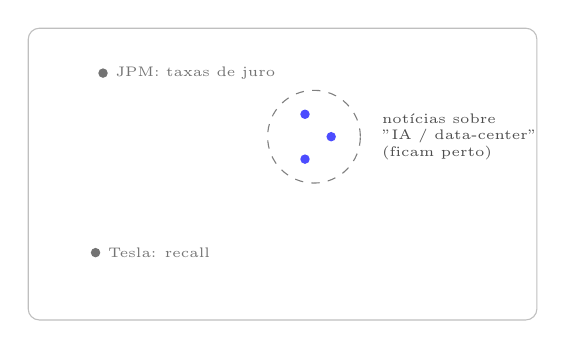
\begin{tikzpicture}[font=\scriptsize, >={Stealth[length=1.6mm]}, scale=0.95]
  \draw[rounded corners, draw=black!25] (-0.2,-0.2) rectangle (6.6,3.7);
  % cluster "IA": tres pontos proximos, rotulados como grupo (sem sobreposicao)
  \fill[blue!70] (3.5,2.55) circle (1.8pt);
  \fill[blue!70] (3.85,2.25) circle (1.8pt);
  \fill[blue!70] (3.5,1.95) circle (1.8pt);
  \draw[dashed,black!50] (3.62,2.25) circle (0.62);
  \node[right, font=\tiny, align=left, black!70] at (4.4,2.25){notícias sobre\\ "IA / data-center"\\ (ficam perto)};
  % nao relacionadas (longe)
  \fill[black!55] (0.7,0.7) circle (1.8pt) node[right=1pt, font=\tiny]{Tesla: recall};
  \fill[black!55] (0.8,3.1) circle (1.8pt) node[right=1pt, font=\tiny]{JPM: taxas de juro};
\end{tikzpicture}
\end{columns}
\vspace{1mm}
\footnotesize \key{Porquê isto importa:} para encontrar notícias passadas \emph{parecidas} com uma nova,
basta procurar os pontos \emph{mais próximos}.
\end{frame}

\begin{frame}{Como medir "perto"? \emph{Similaridade do cosseno}}
\begin{columns}[T]
\column{0.5\textwidth}
\footnotesize
Mede-se o \key{ângulo} entre dois vetores:
\begin{itemize}
  \item ângulo pequeno $\Rightarrow$ cosseno \key{$\approx 1$} (muito parecidos);
  \item ângulo reto $\Rightarrow$ cosseno \key{$\approx 0$} (não relacionados).
\end{itemize}
\vspace{2mm}
Usa-se o ângulo (e não a distância) porque só interessa a \emph{direção} do significado, não o tamanho do
vetor.
\column{0.5\textwidth}
\centering
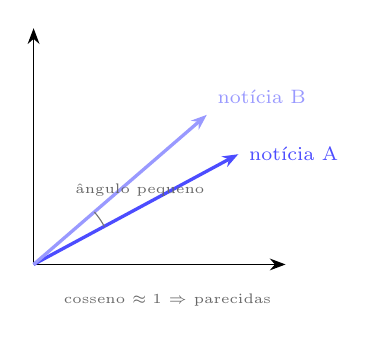
\begin{tikzpicture}[font=\scriptsize, >={Stealth[length=2mm]}, scale=1.0]
  \draw[->] (0,0)--(3.2,0);
  \draw[->] (0,0)--(0,3.0);
  \draw[->, very thick, blue!70] (0,0)--(2.6,1.4) node[right]{notícia A};
  \draw[->, very thick, blue!40] (0,0)--(2.2,1.9) node[above right]{notícia B};
  \draw[black!55] (0.9,0.48) arc (28:41:1.0);
  \node[black!60] at (1.35,0.95){\tiny ângulo pequeno};
  \node[align=center, black!60] at (1.7,-0.45){\tiny cosseno $\approx 1$ $\Rightarrow$ parecidas};
\end{tikzpicture}
\end{columns}
\end{frame}

\begin{frame}{De onde vêm os vetores? \emph{SBERT} (e \emph{Transformer}), em intuição}
\begin{columns}[T]
\column{0.54\textwidth}
\footnotesize
\key{SBERT} (Sentence-BERT) é um modelo \key{já treinado} por outros, que lê uma frase e devolve o seu
vetor de significado. O \key{Transformer} é a arquitetura que o tornou possível (lê a frase inteira e
"presta atenção" às palavras que importam).
\vspace{2mm}

\key{Nesta tese usamo-lo pronto} (inferência): damos-lhe um título, recebemos o vetor. Não o treinamos.
\vspace{2mm}

\emph{Porquê SBERT e não um LLM gigante?} Capta significado, é \key{barato}, \key{reproduzível} e
\key{gratuito}, e dá vetores diretamente comparáveis.
\column{0.46\textwidth}
\centering
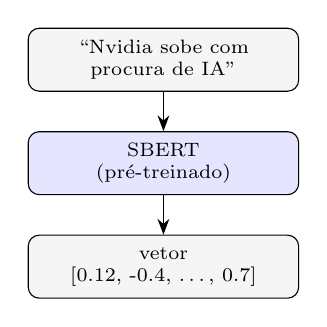
\begin{tikzpicture}[font=\scriptsize, >={Stealth[length=2mm]}, node distance=5mm,
  b/.style={draw, rounded corners, align=center, fill=black!4, text width=3.2cm, minimum height=0.8cm}]
  \node[b] (h){``Nvidia sobe com procura de IA''};
  \node[b, below=of h, fill=blue!10] (m){SBERT \\ \scriptsize (pré-treinado)};
  \node[b, below=of m] (v){vetor \\ \scriptsize [0.12, -0.4, \ldots, 0.7]};
  \draw[->] (h)--(m); \draw[->] (m)--(v);
\end{tikzpicture}
\end{columns}
\end{frame}

\begin{frame}{Ideia-chave 2: estatística para "isto é invulgar?"}
\begin{columns}[T]
\column{0.52\textwidth}
\footnotesize
\key{Média} ($\mu$): o valor típico dos últimos dias.\\
\key{Desvio-padrão} ($\sigma$): o quanto costuma oscilar (a \emph{volatilidade}).\\[2mm]
\key{z-score}: a quantos desvios-padrão está o movimento de hoje:
\[ z=\frac{r-\mu}{\sigma} \]
\emph{Normalizar} pela volatilidade é o truque: a mesma queda de $-3{,}2\%$ é dramática numa ação calma e
banal numa volátil.
\column{0.48\textwidth}
\begin{block}{Exemplo (da tese)}
\footnotesize
Queda de $-3{,}2\%$ hoje:
\begin{itemize}
  \item ação \key{calma} ($\sigma=0{,}40\%$): $z\approx \mathbf{-8{,}1}$ $\Rightarrow$ anomalia clara
  \item ação \key{volátil} ($\sigma=1{,}50\%$): $z\approx \mathbf{-2{,}2}$ $\Rightarrow$ dia normal
\end{itemize}
\vspace{1mm}
Um limiar fixo em \% trataria as duas igual; o z-score não.
\end{block}
\end{columns}
\end{frame}

\begin{frame}{Ideia-chave 3: \emph{retornos} e \emph{event study} (medir o impacto, sem ver o futuro)}
\begin{columns}[T]
\column{0.5\textwidth}
\footnotesize
\key{Log-return}: a variação diária do preço (em \%).\\[1mm]
\key{Event study}: depois de uma notícia, medimos o retorno acumulado a \key{+1, +3 e +5 dias} a partir do
\emph{fecho} do primeiro dia de negociação.
\vspace{2mm}

\key{Anti-lookahead} (regra de ouro de honestidade): só olhamos para \emph{depois} do evento. Nunca usamos o
futuro para "prever". Medimos um \emph{resultado}, não uma previsão.
\column{0.5\textwidth}
\centering
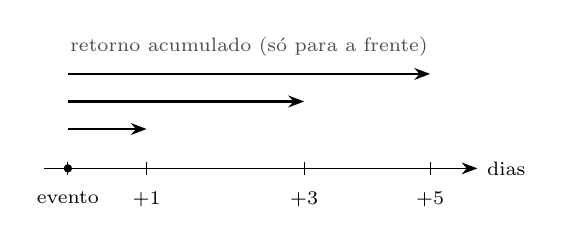
\begin{tikzpicture}[font=\scriptsize, >={Stealth[length=2mm]}]
  \draw[->] (-0.3,0)--(5.2,0) node[right]{dias};
  \foreach \x in {0,1,3} {\draw (\x,0.08)--(\x,-0.08);}
  \filldraw (0,0) circle (1.3pt);
  \node[below=2pt, align=center] at (0,-0.1){\scriptsize evento};
  \node[below=2pt] at (1,-0.1){\scriptsize +1};
  \node[below=2pt] at (3,-0.1){\scriptsize +3};
  \node[below=2pt] at (4.6,-0.1){\scriptsize +5};
  \draw (4.6,0.08)--(4.6,-0.08);
  \draw[->,thick] (0,0.5)--(1,0.5);
  \draw[->,thick] (0,0.85)--(3,0.85);
  \draw[->,thick] (0,1.2)--(4.6,1.2);
  \node[above, black!70] at (2.3,1.3){\scriptsize retorno acumulado (só para a frente)};
\end{tikzpicture}
\end{columns}
\end{frame}

\begin{frame}{Ideia-chave 4: \emph{recuperação} e como se mede (precision@k)}
\begin{columns}[T]
\column{0.54\textwidth}
\footnotesize
\key{Recuperação} (Information Retrieval): ordenar notícias passadas pela semelhança a uma nova e mostrar as
\key{$k$ melhores} (ex.: $k=5$).
\vspace{2mm}

\key{precision@k}: das $k$ recuperadas, que fração é \emph{relevante}? Usamos "mesmo setor" como proxy
automático de relevância.
\vspace{2mm}

Comparamos sempre com \key{baselines} para o número ter significado:
\begin{itemize}
  \item \key{aleatório} (o "chão" sem perícia),
  \item \key{recência} (só as mais recentes),
  \item \key{lexical} (sobreposição de palavras).
\end{itemize}
\column{0.46\textwidth}
\begin{block}{Intuição}
\footnotesize
"Das 5 notícias passadas que mostrei, quantas eram mesmo do mesmo tema?"\\[2mm]
Bater o aleatório e o lexical é a prova de que os \emph{embeddings} acrescentam valor real.
\end{block}
\end{columns}
\end{frame}

\begin{frame}{Ideia-chave 5: explicabilidade (XAI) e confiança}
\begin{columns}[T]
\column{0.5\textwidth}
\footnotesize
\key{Transparente vs caixa-preta:} ou o modelo é interpretável por desenho, ou é opaco e explicamo-lo
\emph{a posteriori} (LIME/SHAP). O CLARION escolhe \key{transparente por desenho}.
\vspace{2mm}

\key{Fidelidade:} a explicação reflete \emph{exatamente} o que o sistema calculou (não é uma aproximação).
\vspace{2mm}

\key{Confiança calibrada:} queremos que o utilizador confie \emph{na medida certa} --- nem ignorar um bom
aviso, nem confiar cegamente. Por isso mostramos \emph{evidência verificável}, não uma narrativa.
\column{0.5\textwidth}
\begin{block}{Raciocínio Baseado em Casos (CBR)}
\footnotesize
A ideia familiar por trás do motor: como um médico que se lembra de \emph{doentes parecidos} do passado.\\[2mm]
\key{Recuperar} casos semelhantes $\to$ \key{reutilizar} o que aconteceu como evidência. Paramos aqui (não
"prevemos").
\end{block}
\end{columns}
\end{frame}

\begin{frame}{Glossário (os termos que vais ouvir)}
\footnotesize
\begin{columns}[T]
\column{0.5\textwidth}
\begin{itemize}
  \item \key{Embedding}: texto $\to$ vetor de significado.
  \item \key{Cosseno}: medida de semelhança (ângulo).
  \item \key{SBERT}: modelo pré-treinado que cria embeddings de frases.
  \item \key{z-score}: nº de desvios-padrão face à norma recente.
  \item \key{Volatilidade}: o quanto uma ação costuma oscilar ($\sigma$).
\end{itemize}
\column{0.5\textwidth}
\begin{itemize}
  \item \key{Event study}: medir o retorno após um evento.
  \item \key{Anti-lookahead}: nunca usar o futuro.
  \item \key{precision@k}: acerto nas $k$ melhores.
  \item \key{Baseline}: método simples de comparação.
  \item \key{XAI / fidelidade}: explicação fiel ao cálculo.
  \item \key{CBR}: raciocínio por casos análogos.
\end{itemize}
\end{columns}
\vspace{2mm}
\centering\footnotesize Tens agora as bases. As próximas partes aplicam \emph{exatamente} estes conceitos à tese.
\end{frame}

\begin{frame}{Fim da Parte 1}
\centering
\vfill
{\Large Já tens as \key{bases de IA} de que esta tese precisa.}\\[4mm]
{\normalsize A seguir: \emph{o problema e a contribuição}, depois \emph{o sistema} (dados, partes, fluxo),
o \emph{código} e a \emph{avaliação}.}
\vfill
\end{frame}

% ====================================================================
\section{O problema}

\begin{frame}{Para quem é? E qual é o problema?}
\begin{columns}[T]
\column{0.55\textwidth}
\footnotesize
\key{Investidor de retalho:} uma pessoa comum que investe (não um profissional).
\vspace{2mm}

O problema é a \key{sobrecarga de informação}: milhares de ações mexem-se e as notícias chegam sem pausa. As
ferramentas que ajudam a interpretar isto são \key{institucionais, opacas, ou ambas}.
\vspace{2mm}

E este investidor é guiado pela \key{atenção}: reage a movimentos extremos e a notícias salientes. Logo, faz
sentido intervir \emph{exatamente nesses momentos}, com \key{contexto e explicação}.
\column{0.45\textwidth}
\centering
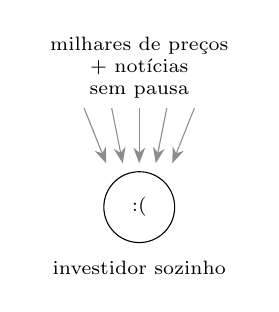
\begin{tikzpicture}[font=\scriptsize,>={Stealth[length=2mm]}]
  \node[align=center,text width=2.6cm] (flood) {milhares de preços\\ $+$ notícias sem pausa};
  \node[draw,circle,below=8mm of flood,minimum size=9mm] (inv) {\scriptsize :(};
  \node[below=1mm of inv,font=\scriptsize]{investidor sozinho};
  \foreach \x in {-1.4,-0.7,0,0.7,1.4} \draw[->,black!45] ($(flood.south)+(\x*0.5,0)$)--($(inv.north)+(\x*0.3,0.1)$);
\end{tikzpicture}\\[1mm]
{\tiny sem as ferramentas que bancos e fundos têm}
\end{columns}
\end{frame}

\begin{frame}{A resposta: dois gatilhos, sempre com explicação}
\centering
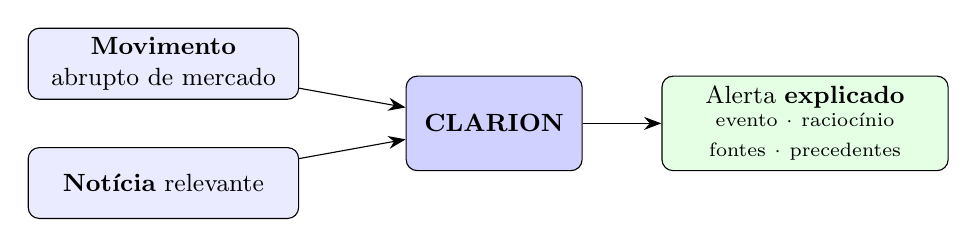
\begin{tikzpicture}[font=\small,>={Stealth[length=2.2mm]},
  t/.style={draw,rounded corners,fill=blue!8,align=center,text width=3.2cm,minimum height=0.9cm},
  s/.style={draw,rounded corners,fill=blue!18,align=center,text width=2.0cm,minimum height=1.2cm},
  o/.style={draw,rounded corners,fill=green!10,align=center,text width=3.4cm,minimum height=1.2cm}]
  \node[t](t1){\textbf{Movimento} abrupto de mercado};
  \node[t,below=6mm of t1](t2){\textbf{Notícia} relevante};
  \node[s] (sys) at ($(t1)!0.5!(t2)+(4.2,0)$){\textbf{CLARION}};
  \node[o,right=1.0cm of sys](out){Alerta \textbf{explicado}\\ \scriptsize evento $\cdot$ raciocínio\\ \scriptsize fontes $\cdot$ precedentes};
  \draw[->](t1)--(sys);\draw[->](t2)--(sys);\draw[->](sys)--(out);
\end{tikzpicture}
\vspace{3mm}

\footnotesize O alerta não é uma notificação seca: traz a \key{cadeia de raciocínio completa}, que o
investidor pode \key{seguir e verificar}.
\end{frame}

\begin{frame}{O que faz --- e o que \key{não} faz}
\begin{columns}[T]
\column{0.5\textwidth}
\begin{block}{\textcolor{good}{Faz}}
\footnotesize
\begin{itemize}
  \item Deteta movimentos invulgares e explica-os.
  \item Para uma notícia, mostra \key{precedentes históricos} reais e o impacto que tiveram.
  \item Expõe toda a evidência (rastreável).
\end{itemize}
\end{block}
\column{0.5\textwidth}
\begin{block}{\textcolor{bad}{Não faz (por desenho)}}
\footnotesize
\begin{itemize}
  \item \textcolor{bad}{$\times$}~Prever preços.
  \item \textcolor{bad}{$\times$}~Trading automático / conselho.
  \item \textcolor{bad}{$\times$}~APIs pagas (só gratuitas).
\end{itemize}
\end{block}
\end{columns}
\vspace{1mm}
\centering\footnotesize É uma escolha de \key{honestidade e defensibilidade}: medir o passado como evidência,
nunca prometer o futuro.
\end{frame}

\begin{frame}{A contribuição: \emph{Engenharia} de IA}
\footnotesize
A contribuição \key{não} é inventar algoritmos. É \key{integrar, aplicar e avaliar criticamente} componentes
existentes num sistema funcional, explicável e reproduzível. Três contribuições concretas:
\begin{enumerate}
  \item Uma \key{metodologia} reproduzível de correlação notícia$\to$impacto (embeddings $+$ event study,
        sem lookahead).
  \item O \key{CLARION}, um sistema de alertas \key{explicável} cuja cadeia de raciocínio é toda exposta ao
        utilizador e \emph{fiel por construção}.
  \item Uma \key{avaliação crítica e honesta} de cada componente em dados reais, contra baselines, com
        limitações reportadas.
\end{enumerate}
\vspace{1mm}
\begin{block}{Defesa em 1 frase}
\scriptsize "Usar modelos e ferramentas existentes \emph{é} o trabalho de engenharia: o valor está no
sistema coerente, explicável e reproduzível, não num algoritmo novo."
\end{block}
\end{frame}

% ====================================================================
\section{O sistema}

\begin{frame}{Arquitetura num relance}
\centering
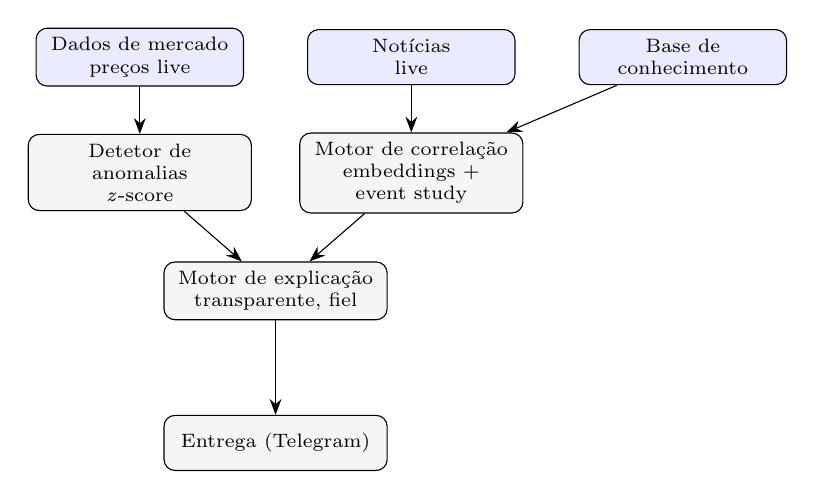
\begin{tikzpicture}[font=\scriptsize,>={Stealth[length=2mm]},
  s/.style={draw,rounded corners,fill=blue!8,align=center,text width=2.4cm,minimum height=0.7cm},
  c/.style={draw,rounded corners,fill=black!4,align=center,text width=2.6cm,minimum height=0.7cm},
  node distance=6mm and 8mm]
  \node[s](md){Dados de mercado\\ \scriptsize preços live};
  \node[s,right=of md](nf){Notícias\\ \scriptsize live};
  \node[s,right=of nf](kb){Base de conhecimento};
  \node[c,below=of md](an){Detetor de anomalias\\ \scriptsize \emph{z}-score};
  \node[c,below=of nf](ce){Motor de correlação\\ \scriptsize embeddings $+$ event study};
  \node[c] (ex) at ($(an)!0.5!(ce)+(0,-1.5)$){Motor de explicação\\ \scriptsize transparente, fiel};
  \node[c,below=1.2cm of ex](tg){Entrega (Telegram)};
  \draw[->](md)--(an);\draw[->](nf)--(ce);\draw[->](kb)--(ce);
  \draw[->](an)--(ex);\draw[->](ce)--(ex);\draw[->](ex)--(tg);
\end{tikzpicture}
\vspace{2mm}

\footnotesize Componentes de \key{responsabilidade única}, ligados por um \key{esquema comum}. Dois gatilhos
convergem num único passo de explicação antes de enviar.
\end{frame}

\begin{frame}{O modelo de dados (os objetos e as relações)}
\centering
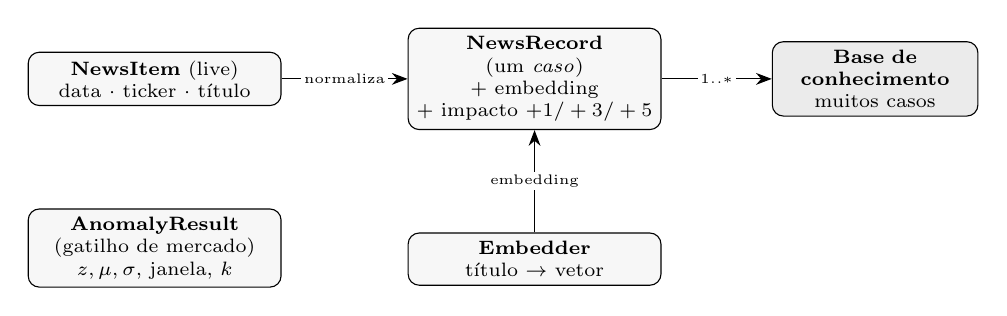
\begin{tikzpicture}[font=\scriptsize,>={Stealth[length=2mm]},
  e/.style={draw,rounded corners,fill=black!3,align=center,text width=3.0cm,inner sep=3pt},
  st/.style={draw,rounded corners,fill=black!8,align=center,text width=2.4cm,inner sep=3pt},
  lbl/.style={midway,font=\tiny,fill=white,inner sep=1pt}]
  \node[e](ni){\textbf{NewsItem} (live)\\ data $\cdot$ ticker $\cdot$ título};
  \node[e,right=1.6cm of ni](nr){\textbf{NewsRecord} (um \emph{caso})\\ $+$ embedding\\ $+$ impacto $+1/+3/+5$};
  \node[st,right=1.4cm of nr](kb){\textbf{Base de}\\ \textbf{conhecimento}\\ muitos casos};
  \node[e,below=1.3cm of nr](emb){\textbf{Embedder}\\ título $\to$ vetor};
  \node[e,below=1.3cm of ni](ar){\textbf{AnomalyResult}\\ \scriptsize (gatilho de mercado)\\ $z,\mu,\sigma$, janela, $k$};
  \draw[->](ni)--node[lbl]{normaliza}(nr);
  \draw[->](nr)--node[lbl]{$1..*$}(kb);
  \draw[->](emb)--node[lbl]{embedding}(nr);
\end{tikzpicture}
\vspace{2mm}

\footnotesize \key{Ideia central:} um \emph{caso} = uma notícia passada $+$ o que aconteceu ao preço a
seguir. \key{NewsItem} (live) e \key{NewsRecord} (histórico) partilham o mesmo esquema, por isso são
diretamente comparáveis.
\end{frame}

\begin{frame}{Os componentes e o que cada um faz}
\centering\scriptsize
\begin{tabular}{@{}p{3.0cm} p{4.0cm} p{4.2cm}@{}}
\toprule
\textbf{Componente} & \textbf{Responsabilidade} & \textbf{Entrada $\to$ saída} \\
\midrule
Dados de mercado & preços, log-returns & ticker $\to$ retornos diários \\
Notícias & obter e normalizar & ticker $\to$ NewsItem(s) \\
Embedder & título $\to$ vetor & título $\to$ embedding \\
Base de conhecimento & guardar/recuperar casos & título $\to$ top-$k$ casos \\
Detetor de anomalias & sinalizar movimento invulgar & retornos $\to$ AnomalyResult \\
Motor de correlação & cosseno $+$ event study & título, KB $\to$ precedentes $+$ impacto \\
Motor de explicação & montar o alerta fiel & objetos $\to$ texto do alerta \\
Entrega & enviar ao utilizador & texto $\to$ Telegram \\
\bottomrule
\end{tabular}
\vspace{1mm}

\footnotesize Cada componente tem \key{uma} responsabilidade: é o que permite testar offline e trocar peças.
\end{frame}

\begin{frame}{Os dois gatilhos, lado a lado}
\footnotesize
\textbf{Gatilho de mercado:}
\begin{center}
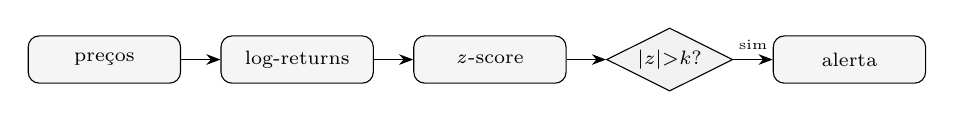
\begin{tikzpicture}[font=\scriptsize,>={Stealth[length=1.8mm]},node distance=5mm,
  b/.style={draw,rounded corners,fill=black!4,align=center,text width=1.7cm,minimum height=0.6cm},
  d/.style={draw,diamond,aspect=2,fill=black!5,inner sep=1pt,align=center,text width=0.9cm}]
  \node[b](a){preços};\node[b,right=of a](b){log-returns};\node[b,right=of b](c){\emph{z}-score};
  \node[d,right=of c](e){$|z|{>}k$?};\node[b,right=of e](f){alerta};
  \draw[->](a)--(b);\draw[->](b)--(c);\draw[->](c)--(e);\draw[->](e)--node[above,font=\tiny]{sim}(f);
\end{tikzpicture}
\end{center}
\textbf{Gatilho de notícia:}
\begin{center}
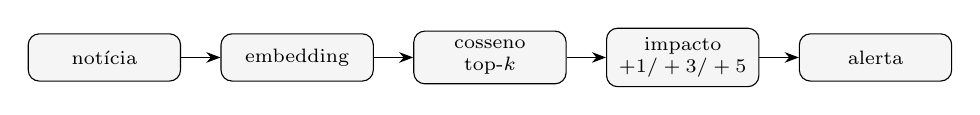
\begin{tikzpicture}[font=\scriptsize,>={Stealth[length=1.8mm]},node distance=5mm,
  b/.style={draw,rounded corners,fill=black!4,align=center,text width=1.7cm,minimum height=0.6cm}]
  \node[b](a){notícia};\node[b,right=of a](b){embedding};\node[b,right=of b](c){cosseno\\ top-$k$};
  \node[b,right=of c](d){impacto\\ $+1/+3/+5$};\node[b,right=of d](e){alerta};
  \draw[->](a)--(b);\draw[->](b)--(c);\draw[->](c)--(d);\draw[->](d)--(e);
\end{tikzpicture}
\end{center}
\vspace{1mm}
\centering Ambos terminam no \key{motor de explicação}, que monta o alerta a partir dos objetos calculados.
\end{frame}

% ====================================================================
\section{Os dados}

\begin{frame}{Que dados? Duas camadas}
\begin{columns}[T]
\column{0.5\textwidth}
\begin{block}{Histórica (offline)}
\footnotesize
\key{FNSPID}: notícias alinhadas a preços diários.\\[1mm]
\emph{Data card:} 15 ações grandes, 5 setores (tecnologia, banca, energia, saúde, consumo), 2018--2023.
Licença CC BY-SA 4.0 (atribuição obrigatória).
\end{block}
\column{0.5\textwidth}
\begin{block}{Live}
\footnotesize
Preços (yfinance) $+$ notícias (Finnhub/RSS), só APIs \key{gratuitas}.\\[1mm]
A avaliação usa um corpus \key{real e recente} (3\,714 títulos) construído pelo mesmo processo; o FNSPID
multi-ano fica como trabalho futuro.
\end{block}
\end{columns}
\vspace{1mm}
\centering\footnotesize As duas camadas partilham o \key{mesmo esquema} (data, ticker, título) $\Rightarrow$
o novo é comparável com o histórico.
\end{frame}

\begin{frame}[fragile]{A estrutura de pastas (o repositório)}
\footnotesize Onde vive cada coisa:
\begin{verbatim}
DIMEIA/
  thesis/        a dissertacao (LaTeX, 6 capitulos)
  src/           o sistema (um pacote por componente)
  data/samples/  amostras pequenas (CSV, JSONL)
  scripts/       dados, figuras, avaliacao, build
  slides/        slides de defesa + este guia
  docs/          documentacao e provas de rigor
\end{verbatim}
\footnotesize Os dados grandes \key{não} são versionados (recriados por script); só ficam pequenas amostras.
\end{frame}

\begin{frame}[fragile]{Os dados a olho: notícias (CSV) e um caso (JSON)}
\scriptsize \key{Notícias de entrada} (\texttt{news\_sample.csv}) --- três colunas:
\begin{verbatim}
date,ticker,headline
2023-01-09,AAPL,Apple expands services revenue as iPhone demand...
2023-05-25,NVDA,Nvidia guidance surges on soaring demand for AI...
\end{verbatim}
\key{Um "caso" na base de conhecimento} (\texttt{kb\_sample.jsonl}, uma linha):
\begin{verbatim}
{ "date": "2023-01-09", "ticker": "AAPL",
  "headline": "Apple expands services revenue...",
  "impacts": { "1": 0.0045, "3": 0.0250, "5": 0.0445 },
  "embedding": [0.0, 0.0, ..., 0.333]   // 64 numeros }
\end{verbatim}
\end{frame}

\begin{frame}{O JSON de um caso, campo a campo}
\footnotesize
\begin{itemize}
  \item \key{date}, \key{ticker}, \key{headline}: a notícia (igual ao esquema live).
  \item \key{impacts}: o que o preço fez \key{depois} --- retorno acumulado a $+1$, $+3$ e $+5$ dias
        (ex.: $+0{,}45\%$, $+2{,}50\%$, $+4{,}45\%$). \emph{Esta é a "etiqueta" de evidência.}
  \item \key{embedding}: o vetor de significado do título (aqui 64 números do baseline; com SBERT seriam
        centenas). É o que permite comparar por cosseno.
\end{itemize}
\vspace{1mm}
\centering\footnotesize Um caso junta as \key{três coisas} de que o sistema precisa: \emph{o que se disse},
\emph{o que aconteceu} e \emph{como comparar}.
\end{frame}

\begin{frame}{Como nasce um caso (alinhamento $+$ impacto, sem lookahead)}
\centering
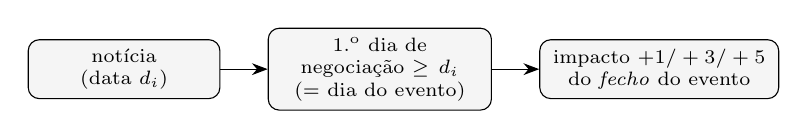
\begin{tikzpicture}[font=\scriptsize,>={Stealth[length=2mm]},node distance=6mm]
  \node[draw,rounded corners,fill=black!4,align=center,text width=2.2cm](n){notícia\\ (data $d_i$)};
  \node[draw,rounded corners,fill=black!4,align=center,text width=2.6cm,right=of n](e){1.\textsuperscript{o} dia de negociação $\ge d_i$\\ \scriptsize (= dia do evento)};
  \node[draw,rounded corners,fill=black!4,align=center,text width=2.8cm,right=of e](i){impacto $+1/+3/+5$\\ \scriptsize do \emph{fecho} do evento};
  \draw[->](n)--(e);\draw[->](e)--(i);
\end{tikzpicture}
\vspace{2mm}

\footnotesize
\begin{itemize}
  \item Mede-se a partir do \key{fecho} (não da abertura): não se credita um salto já no preço de abertura.
  \item Só se olha para a \key{frente} (anti-lookahead): é \emph{evidência} do que aconteceu, não previsão.
  \item Sem preços alinhados, ou janela fora dos dados $\Rightarrow$ a notícia é descartada (não inventada).
\end{itemize}
\end{frame}

\begin{frame}{Fim das Partes 2--4}
\centering\vfill
{\Large Já sabes \key{o problema}, \key{o sistema} e \key{os dados}.}\\[4mm]
{\normalsize A seguir: \emph{o código módulo a módulo} (linha a linha) e o \emph{workflow ponta a ponta}
com exemplos reais.}
\vfill
\end{frame}

% ====================================================================
\section{O código}

\begin{frame}{O código num relance}
\footnotesize
\begin{itemize}
  \item \key{Um pacote por componente} (mercado, deteção, correlação, base de conhecimento, explicação,
        entrega). Cada um faz \emph{uma} coisa.
  \item \key{Lógica pura separada de I/O}: os cálculos (z-score, cosseno, impacto) não precisam de rede nem
        do modelo pesado $\Rightarrow$ testam-se offline e rápido.
  \item \key{Programado a interfaces}: o \texttt{Embedder} é abstrato, com 2 implementações trocáveis.
\end{itemize}
\vspace{1mm}
\centering\footnotesize Nos slides seguintes: cada módulo com um \emph{snippet simplificado mas fiel}, linha
a linha, e um exemplo concreto de valores.
\end{frame}

\begin{frame}[fragile]{Detetor de anomalias --- o \emph{z}-score}
\scriptsize
\begin{verbatim}
def detect_latest(returns, window=20, threshold=3.0):
    recent = returns[-window-1 : -1]     # 20 dias ANTERIORES (sem hoje)
    mu, sigma = mean(recent), std(recent)
    z = (returns[-1] - mu) / sigma       # quantos desvios-padrao e' hoje
    return AnomalyResult(is_anomaly = abs(z) > threshold,
                         z_score=z, mean=mu, std=sigma, window=window, ...)
\end{verbatim}
\footnotesize
\begin{itemize}
  \item \key{recebe} a série de retornos; \key{devolve} um \texttt{AnomalyResult} (decisão $+$ todas as
        quantidades).
  \item \key{recent}: só dias \emph{antes} de hoje $\Rightarrow$ \key{sem lookahead}.
  \item \key{Exemplo (TSLA):} $\mu=-0{,}92\%$, $\sigma=2{,}73\%$, hoje $=+19{,}82\% \Rightarrow z=+7{,}61
        \Rightarrow$ anomalia.
\end{itemize}
\end{frame}

\begin{frame}[fragile]{Similaridade do cosseno $+$ top-$k$}
\scriptsize
\begin{verbatim}
def cosine_similarities(query, matrix):     # query: 1 vetor; matrix: N vetores
    return (matrix @ query) / (row_norms(matrix) * norm(query))

def top_k_similar(query, matrix, k=5):
    sims = cosine_similarities(query, matrix)
    return indices_of_largest(sims, k)      # os k mais parecidos (+ score)
\end{verbatim}
\footnotesize
\begin{itemize}
  \item \key{recebe} o vetor da notícia nova e a matriz de vetores da KB; \key{devolve} os índices dos
        \key{$k$ mais semelhantes} e o seu score (0 a 1).
  \item \texttt{matrix @ query} é o produto interno; dividir pelas normas dá o \key{cosseno} (o ângulo).
  \item \key{Exemplo:} para a consulta da Nvidia, os 5 maiores scores apontam para notícias de chips de IA.
\end{itemize}
\end{frame}

\begin{frame}[fragile]{Event study --- o impacto pós-evento}
\scriptsize
\begin{verbatim}
def post_event_returns(close, event_idx, horizons=(1,3,5)):
    p0 = close[event_idx]                      # fecho do dia do evento
    return { h: close[event_idx + h]/p0 - 1    # retorno acumulado a +h dias
             for h in horizons }
\end{verbatim}
\footnotesize
\begin{itemize}
  \item \key{recebe} a série de fechos e a posição do evento; \key{devolve} \texttt{\{1:.., 3:.., 5:..\}}.
  \item Mede sempre \key{para a frente}, a partir do \key{fecho} ($p_0$). Se faltar dados $\Rightarrow$ NaN
        (não inventa).
  \item \key{Exemplo (AAPL):} $+1$d $=+0{,}45\%$, $+3$d $=+2{,}50\%$, $+5$d $=+4{,}45\%$.
\end{itemize}
\end{frame}

\begin{frame}[fragile]{Embedder --- uma interface, duas implementações}
\scriptsize
\begin{verbatim}
class Embedder(Protocol):           # "contrato": tem dim e encode()
    dim: int
    def encode(self, texts) -> matriz (n, dim): ...

class HashingEmbedder:   # baseline SEM dependencias (reprodutivel, p/ testes)
class SbertEmbedder:     # SBERT pre-treinado (a abordagem da tese, inferencia)
\end{verbatim}
\footnotesize
\begin{itemize}
  \item Ambos cumprem o mesmo contrato $\Rightarrow$ a KB e a recuperação funcionam com qualquer um.
  \item Por isso podemos \key{comparar} MiniLM vs MPNet vs lexical de forma \key{justa} (só troca o embedder).
  \item O \texttt{HashingEmbedder} permite correr tudo \key{sem a stack pesada} (torch).
\end{itemize}
\end{frame}

\begin{frame}[fragile]{Base de conhecimento --- construir e recuperar}
\scriptsize
\begin{verbatim}
class HistoricalKB:
    def build(news, prices, embedder):      # 1 "caso" por noticia
        for (date, ticker, headline) in news:
            e = first_trading_day >= date            # alinhar ao evento
            impacts = post_event_returns(prices[ticker], e)
            emb     = embedder.encode([headline])[0]
            add NewsRecord(date, ticker, headline, impacts, emb)

    def find_precedents(query_text, embedder, top_k=5):
        q = embedder.encode([query_text])[0]
        return top_k_similar(q, all_embeddings)  # -> [(NewsRecord, score), ...]
\end{verbatim}
\footnotesize
\key{build} (offline) cria a memória de casos; \key{find\_precedents} (live) devolve os mais parecidos com a
notícia nova. É o \key{núcleo} do sistema (raciocínio baseado em casos).
\end{frame}

\begin{frame}[fragile]{Motor de explicação --- o alerta \emph{fiel}}
\scriptsize
\begin{verbatim}
def explain_news_impact(ticker, headline, precedents, horizon=1):
    avg = mean(impacto[horizon] de cada precedente)   # so a media
    linhas = [f"impacto medio {horizon}d: {avg:.2%}"]
    for (rec, score) in precedents:                    # mostra CADA precedente
        linhas += [f"{rec.date} {rec.ticker} (sim {score:.2f}) {rec.impacts[...]:.2%}"]
    linhas += ["Nota: resultado passado, NAO e' previsao."]
    return "\n".join(linhas)
\end{verbatim}
\footnotesize
\begin{itemize}
  \item O texto é montado \key{a partir dos próprios objetos calculados} $\Rightarrow$ \key{fiel por
        construção} (não pode divergir da lógica).
  \item Mostra \key{cada} precedente (não só a média) e termina sempre com o \key{aviso de não-previsão}.
\end{itemize}
\end{frame}

% ====================================================================
\section{Workflow}

\begin{frame}{Workflow (1/3): construir a memória, uma vez (offline)}
\centering
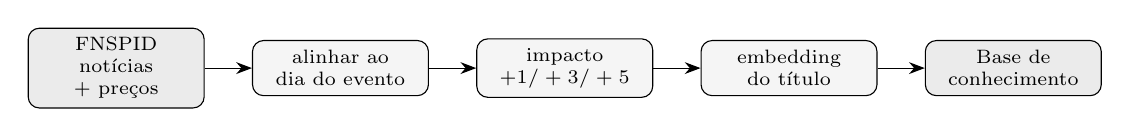
\begin{tikzpicture}[font=\scriptsize,>={Stealth[length=2mm]},node distance=6mm,
  b/.style={draw,rounded corners,fill=black!4,align=center,text width=2.0cm,minimum height=0.7cm},
  db/.style={draw,rounded corners,fill=black!8,align=center,text width=2.0cm,minimum height=0.7cm}]
  \node[db](f){FNSPID\\ notícias $+$ preços};
  \node[b,right=of f](al){alinhar ao\\ dia do evento};
  \node[b,right=of al](im){impacto\\ $+1/+3/+5$};
  \node[b,right=of im](em){embedding\\ do título};
  \node[db,right=of em](kb){Base de\\ conhecimento};
  \draw[->](f)--(al);\draw[->](al)--(im);\draw[->](im)--(em);\draw[->](em)--(kb);
\end{tikzpicture}
\vspace{3mm}

\footnotesize Resultado: uma base de \key{casos} (\emph{notícia $\to$ impacto $+$ vetor}), pronta a ser
consultada. Feita \key{uma vez}; depois é só usar.
\end{frame}

\begin{frame}{Workflow (2/3): gatilho de mercado --- TSLA, 24-10-2024 (real)}
\footnotesize
\begin{enumerate}
  \item Preços live $\to$ log-return de hoje: \key{$r=+19{,}82\%$} (movimento de $\approx +22\%$).
  \item Janela dos 20 dias \key{anteriores}: \key{$\mu=-0{,}92\%$}, \key{$\sigma=2{,}73\%$}.
  \item $z = (19{,}82-(-0{,}92))/2{,}73 = \mathbf{+7{,}61}$.
  \item $|7{,}61|>3 \Rightarrow$ \key{anomalia}. O alerta expõe $r,\mu,\sigma$, janela e limiar, e traduz:
        \emph{"$\approx 7{,}6\times$ a oscilação diária típica desta ação"}.
\end{enumerate}
\vspace{1mm}
\begin{block}{Porque é convincente}
\scriptsize Reprodutível por \texttt{scripts/evaluate\_anomaly.py} (janela fixa). O mesmo valor sai sempre.
\end{block}
\end{frame}

\begin{frame}[fragile]{Workflow (3/3): gatilho de notícia --- Nvidia (real)}
\scriptsize
Consulta: \emph{``Nvidia raises guidance on surging demand for AI data-centre accelerators''} $\to$ embedding
$\to$ cosseno top-5 $\to$ alerta:
\begin{verbatim}
Alerta NVDA  | impacto medio 1 dia: -1,97%
 - MSFT  (sim 0.68)  +1d -3,46%  "Qualcomm debuts AI data center chips..."
 - NVDA  (sim 0.68)  +1d -1,64%  "Qualcomm debuts AI data center chips..."
 - META  (sim 0.68)  +1d -2,65%  "Qualcomm debuts AI data center chips..."
 - GOOGL (sim 0.64)  +1d -0,46%  "...bigger than Nvidia..."
 - NVDA  (sim 0.58)  +1d -1,64%  "...NVIDIA..."
Nota: precedentes por semelhanca; impacto observado, NAO previsao.
\end{verbatim}
\footnotesize Todos falam de \key{chips de IA para data-center}, mesmo vindo de empresas diferentes
(\key{cross-ticker}): a recuperação é por \key{significado}, não pelo nome da empresa.
\end{frame}

\begin{frame}{A nota mais honesta (e a pergunta certa do júri)}
\footnotesize
\begin{block}{Um título \emph{positivo} deu precedentes \emph{negativos} ($-1{,}97\%$). Engana?}
A semelhança capta o \key{tema} ("chips de IA"), \key{não a direção} (o sentimento). Por isso um título
positivo pode recuperar um \emph{cluster} de ameaça competitiva, com desfechos negativos.
\end{block}
A média é \key{evidência sobre um tema}, \key{não uma previsão} para este caso. É por isso que o alerta:
\begin{itemize}
  \item mostra sempre os precedentes \key{um a um} (não só a média);
  \item termina com o \key{aviso de não-previsão} (evita a \emph{sobre-confiança}).
\end{itemize}
\centering\footnotesize Melhorias futuras: de-duplicar precedentes e \key{sinalizar quando o cluster discorda
na direção}.
\end{frame}

\begin{frame}{Fim das Partes 5--6}
\centering\vfill
{\Large Já viste \key{o código} e o \key{workflow} com exemplos reais.}\\[4mm]
{\normalsize A seguir: \emph{a avaliação} (o que cada número significa), as \emph{decisões de desenho},
o \emph{"e se mudássemos\ldots?"} e as \emph{perguntas do júri}.}
\vfill
\end{frame}

\end{document}
